% -----------------------------------------------------------------------------
\section{Purpose}
% -----------------------------------------------------------------------------
% Synthetic biology aims to apply engineering principles such as standardization, modularity, and design abstraction to molecular biology.  However, synthetic biology still faces substantial challenges, including long development times, high rates of failure, and poor reproducibility. 

% The Synthetic Biology Open Language is intended to help synthetic biologists collaborate by allowing them to exchange designs in a standardized data format.  In addition, the SBOL data model systematically describes the essential details of a design that are required for researchers to reproduce each other's designs in the laboratory.  The purpose of the Synthetic Biology Open Language is to aid collaboration between researchers, improve scientific reproducibility, and to speed the research and development of technologies based on synthetic biology.

% Below is my revision. Any thoughts? - Nic

Synthetic biology builds upon the techniques and successes of genetics, molecular biology and metabolic engineering by applying engineering principles to the design of biological systems. These principles include standardization, modularity, and design abstraction. The field still faces substantial challenges, including long development times, high rates of failure, and poor reproducibility. A common factor of these challenges is the exchange of information about designed systems between laboratories. When designing a synthetic system,  synthetic biologists need to exchange information about multiple types of molecules and their planned roles in the design. Often the functional role may be associated with another type of molecule entirely, such as a small chemical, a DNA, an RNA or a Protein molecule. An example is an DNA sequence that is transcribed into a messenger RNA that contains an encoded microRNA binding site, and the messenger RNA in turn being translated into a protein molecule which is a transcription factor binding protein. Functionally the representation of the products of the designed DNA sequence need to describe the role of microRNA binding to the messenger RNA leading to possible  degradation, the functional consequence of the transcription factor protein being absent leading to repression of expression of another gene and the kinetic information associated with these different elements so they can be mathematically modeled. The DNA sequence itself is thus one or two steps removed from the functional role of the designed device or circuit. 

SBOL has been designed as a standard to support synthetic biology, filling a need not satisfied by other pre-existing standards. Previous file formats such as GenBank and SwissProt represent sequence information based upon annotation of sequence features - they do not represent the functional roles or consequences of these sequences. Systems Biology Markup Language (SBML) represents reactions, pathways, and models, but does not typically represent the associated sequences.  Kinetic information may be present in SBML~\cite{SBML} or mass conservation laws in other systems such as the COBRA Toolbox~\cite{COBRA}. Synthetic Biology needs a structured standard with defined ways on how to represent relevant molecules and their functional roles within the designed system, standardized rules on how such information is encoded in the file and the means to enable exchange of such data between participating laboratories as part of publications. 

To help address these challenges, the Synthetic Biology Open Language (SBOL) Standard introduces a standardized format for the electronic exchange of information describing the structural and functional aspects of biological designs. 
The standard is designed to support the development of explicit and unambiguous data models of biological designs through the use of a well defined model on how to represent the component molecules, and their structural and functional roles in a systematic fashion. 
The standard further describes rules and best practices on how to include, develop and populate this format with relevant information of essential design details. 
Because the standard itself can represent information from other sources for sequence representations, reaction information and ontologies to represent biological design information, the standard uses modern information exchange techniques such as Universal Resource Identifiers (URIs). This permits the reuse of existing information without the need to repeat it, thus avoiding both redundancy and likely future information decay within shared files. 
The ultimate utility of URIs in the SBOL Standard is the ability to support flexible annotation with appropriate metadata while associating an authority with that annotation. 
The definition of the data model and associated format, the rules on the addition of data within the format and the representation of this in electronic data files are intended to make the SBOL Standard a useful means of promoting global data exchange between laboraties and between software programs.

\Ctodo{Need to make clear that this replaces SBOL 1.1 and all future work should use SBOL 2.0.}

This document presents the second version of SBOL.
The previous version 1.1 of the SBOL standard focused on representing the structural aspects of genetic designs. 
Users of the standard were able to use it to echange information on DNA designs but could not represent molecules other than DNA or represent the functional aspects of their designs beyond the DNA sequences. 
To serve as an effective medium for the computational exchange of genetic designs, SBOL must be extended to capture more aspects of a designed system, including both structural and functional information, and the composition of complex structural and functional designs by combining simpler parts. 
The SBOL 2.0 data model defined in this specification thus extends the prior model to provide for addressing the most pressing needs for expanding SBOL Version 1.1:

\begin{itemize}

\item represent structural components of a biological design, including DNA, RNA, proteins, small molecules and other physical components

\item describe behavioral aspects of a biological design, the intended or expected interactions and dynamic behavior

\item associate structure and function together, so that a single design can be understood both in terms of its structure and its behavior

\item support rich annotations of all components, so that data required to describe a design, but not formalized in this specification can be safely exchanged

\end{itemize}

\begin{figure}
\centering
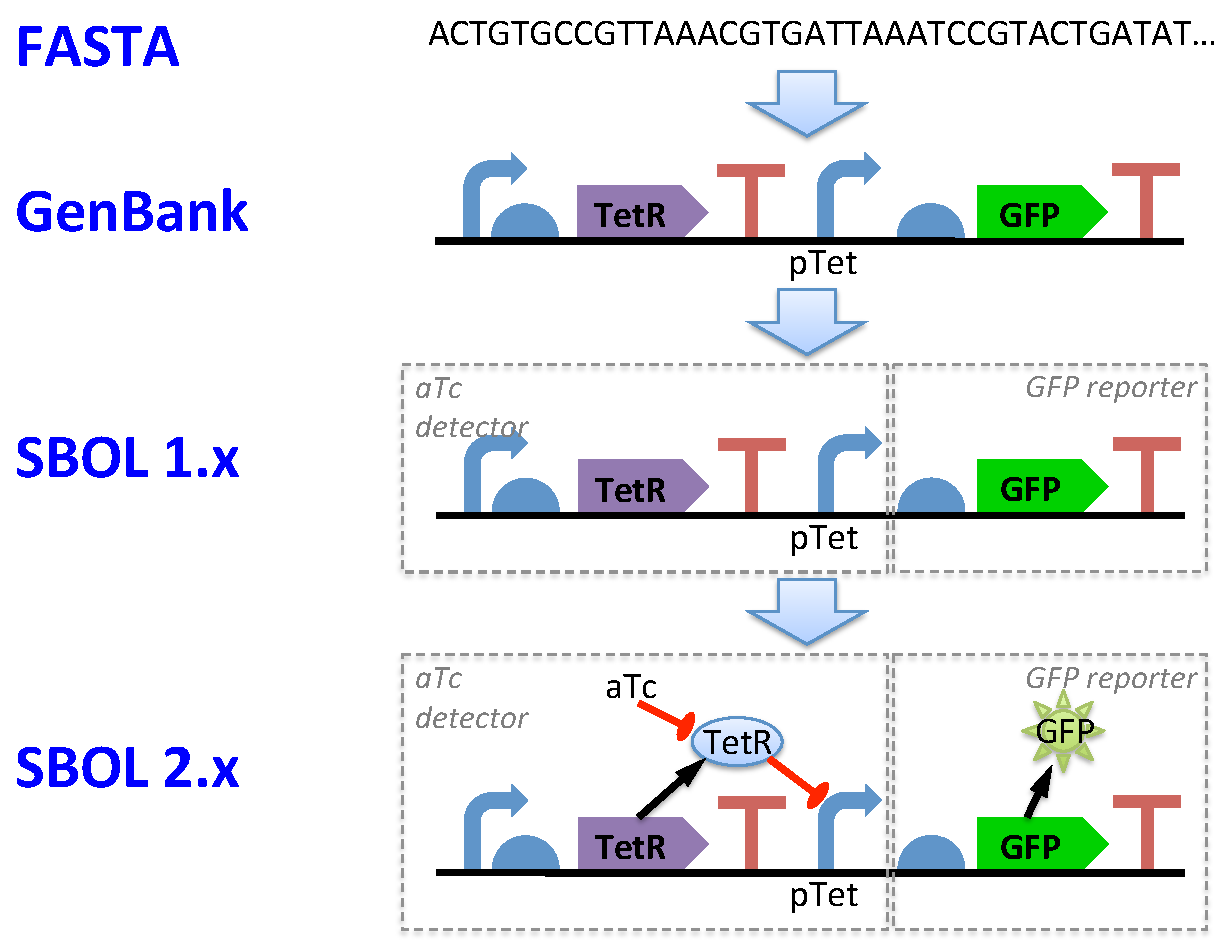
\includegraphics[width=5in]{images/format-comparison.pdf}
\caption{SBOL 2.0 extends prior formats to represent both structure and function of a genetic design in a single model.}
\end{figure}

\Rtodo{Please review this new figure}

Taken together, these capabilities allow SBOL sufficient expressivity to support the description and exchange of hierarchical, modular representations of both the intended structure and function of designed biological systems.

To address the need for functional descriptions in SBOL, the proposed data model adds classes for modules, interactions, and models. These classes provide a firm basis for functional representation in SBOL without going so far as to create a new standard for mathematically modeling biology, as there already exist several established languages for doing so, from the Systems Biology Markup Language (SBML)~\cite{SBML} to CellML~\cite{CellML} and even MatLab~\cite{matlab}. Rather, these classes enable users of SBOL to group components that function together, describe the basic qualitative interactions between these components, and document references to standard mathematical models that are external to SBOL and that provide more detailed descriptions of component function. In other words, a module gathers together a set of component instantiations, a set of interactions between these component instantiations, and a set of references to external models that are expected to be consistent with the module's interactions.

\Rtodo{Added next two paragraphs to address queries from Mike B.  -JSB}

The SBOL 2.0 specification also adds a number of measures to simplify adoption and validation of compatibility with the standard.
First, the specification explicitly incorporates its serialization format into the specification, whereas SBOL 1.1 used an implicit standard tied to a reference implementation.
Second, the specification includes a set of validation rules for determining compatibility of a document with SBOL 2.0, most of which are machine-verifiable.
Finally, the specification includes a set of recommended best-practices likely to allow a tool to take best advantage of the standard and other compatible tools.

Care has been taken to ensure that SBOL 2.0 is backward-compatible with SBOL 1.x.  
The generalization of the data model does mean that many names have changed and thus an SBOL 1.x file is not a valid SBOL 2.0 file.
There is, however, a direct mapping from the SBOL 1.x data model into the SBOL 2.0 data model, making it simple to automatically ``upgrade'' any SBOL 1.x file into and SBOL 2.0 file.

The SBOL standard has been developed in collaboration between both ``wet'' bench scientists and ``dry'' scientific modelers and tool designers active within the Synthetic Biology community. 
As with the earlier SBOL 1.1 standard this community (open for any practitioner to join) has met to discuss, argue and agree upon needs that the SBOL standard should address. 
This information has then been used by developers within our community to design, develop and test a specification of the standard. The specification has been tested by the community through several iterations for the ability to represent a wide range of synthetic biology design projects, as well as, the ability to share designs between different laboratories. 
The standard has also been used to develop software tools that employ the standard for developing and sharing synthetic design projects. 
The publication of this specification is intended to make these capabilities more widely accessible to the community of potential developers and users.